\documentclass[12pt,a4paper]{article}
\usepackage[utf8]{inputenc}
\usepackage[spanish]{babel}
\usepackage{graphicx}
\usepackage{geometry}
\usepackage{float}
\usepackage{listings}
\usepackage{xcolor}

\geometry{left=2.5cm,right=2.5cm,top=2.5cm,bottom=2.5cm}

\definecolor{backcolour}{rgb}{0.95,0.95,0.92}
\lstdefinestyle{terminal}{
    backgroundcolor=\color{backcolour},
    basicstyle=\ttfamily\scriptsize, 
    breakatwhitespace=false,         
    breaklines=true,                 
    captionpos=b,                    
    keepspaces=true,                 
    showspaces=false,                
    showstringspaces=false,
    showtabs=false,                  
    tabsize=2,
    xleftmargin=0.02\textwidth,
    xrightmargin=0.02\textwidth
}
\lstset{style=terminal}

\title{Reporte Técnico: Análisis Estadístico y Modelado de Ventas \\ \Large Farmacias Cruz Morada}
\author{Computación Paralela y Distribuida}
\date{\today}

\begin{document}

\maketitle
\tableofcontents
\newpage

\section{Descripción de la Solución Implementada}
Para resolver el desafío de analizar el archivo \texttt{ventas\_completas.csv} (que contiene más de 3.2 millones de registros) de la cadena Cruz Morada, se implementó una solución computacional escalable utilizando procesamiento paralelo.

\textbf{Justificación de la Técnica:} Dado que cargar un archivo tan masivo directamente a la memoria RAM con herramientas tradicionales (como \texttt{pandas}) provocaría colapsos por falta de memoria (Out-of-Memory), se optó por una lectura particionada o \textit{chunking}. La ejecución se realiza en bloques de 64MB, asignando cada partición lógica a uno de los 10 hilos (workers) disponibles en el procesador.
Además, cumpliendo con la estricta política de reproducibilidad, se garantiza el determinismo del programa inyectando una semilla global mediante la variable de entorno \texttt{CPYD\_SEED=42}.

\section{Justificación de las Librerías Estadísticas Utilizadas}
Para asegurar un rigor metodológico excepcional, se utilizaron las siguientes librerías de Python, consideradas estándares industriales en la ciencia de datos:
\begin{itemize}
    \item \textbf{Dask:} Utilizado para el paralelismo nativo. Es una extensión de Pandas que permite procesar \textit{dataframes} que exceden la capacidad de la memoria RAM.
    \item \textbf{SciPy (\texttt{scipy.stats}):} Se seleccionó para las pruebas de normalidad (Shapiro-Wilk, Kolmogorov-Smirnov), independencia (Chi-cuadrado) y comparación de medianas (Kruskal-Wallis, Mann-Whitney U). Provee implementaciones altamente optimizadas y matemáticamente exactas de estos contrastes de hipótesis.
    \item \textbf{Statsmodels:} Empleado para la regresión lineal (OLS) y sus diagnósticos. A diferencia de \texttt{scikit-learn} (enfocado puramente en predicción \textit{machine learning}), \texttt{statsmodels} está diseñado explícitamente para la \textit{inferencia estadística}, ofreciendo tablas detalladas de coeficientes, p-values, errores estándar, y tests robustos (Breusch-Pagan, Durbin-Watson, VIF).
\end{itemize}

\section{Fase 1: Preprocesamiento y Limpieza}
La consola muestra la ejecución del planificador:

\begin{lstlisting}[caption={Comando inicial de ejecución}]
[Paso 1/4] Preprocesamiento y limpieza de datos (paralelo con Dask)...
[Paralelo] Planificador multihilo con 10 workers.
[Determinismo] Semilla configurada desde CPYD_SEED: 42
\end{lstlisting}

\subsection{Tratamiento de Valores Faltantes}
Para abordar posibles valores faltantes en la columna \texttt{PORCENTAJE DESCUENTO}, se llevó a cabo una prueba de independencia entre si el valor es nulo y el CANAL de venta, con el fin de discernir si el mecanismo era MCAR (Missing Completely At Random) o MAR (Missing At Random). En la muestra de 50,000 registros, se detectó un $0.0000\%$ de nulos. Se decidió rellenar aquellos que pudieran faltar en la totalidad con $0.0$, asumiendo que la ausencia de registro de descuento equivale a que no se aplicó ninguno.
Asimismo, 2,876 registros de edades presentaban inconsistencias lógicas. Se optó por una imputación por la mediana (49.9 años) para no alterar la distribución, ya que la media se ve afectada fuertemente por extremos.

\subsection{Detección de Outliers (Valores Atípicos)}
Se empleó el método del Rango Intercuartílico (IQR), ya que es un estimador robusto frente a distribuciones asimétricas (a diferencia del Z-Score, que asume normalidad).

\begin{lstlisting}[caption={Salida del detector de Outliers}]
Detección de outliers en MONTO APLICADO (método IQR):
  Rango aceptable: [-4,562.50, 23,929.50]
  Outliers detectados: 149,377 (4.61%)
  Decisión: se marcan pero no se eliminan; corresponden a compras 
  reales de alto valor (medicamentos especializados), no errores.
\end{lstlisting}

\section{Fase 2: Análisis Exploratorio Estadístico (EDA)}
En esta fase se caracterizan las variables, comenzando por las métricas descriptivas calculadas en paralelo. 

\begin{lstlisting}[caption={Estadísticas Descriptivas (Ajustado para legibilidad)}]
Media    UNIDADES: 1.0  %DESC: 0.3920  MONTO: 1.017e+04  EDAD: 49.57
DesvStd  UNIDADES: 0.0  %DESC: 0.1080  MONTO: 1.445e+04  EDAD: 16.72
Minimo   UNIDADES: 1.0  %DESC: 0.0000  MONTO: 1.500e+01  EDAD: 0.005
Maximo   UNIDADES: 1.0  %DESC: 1.0000  MONTO: 2.264e+05  EDAD: 109.8
Asimetria               %DESC: 0.2969  MONTO: 9.060      EDAD: 0.241
\end{lstlisting}
*(Nota técnica: UNIDADES posee una varianza de 0, lo que indica que toda transacción de la base de datos se registró como 1 sola unidad).*

\subsection{Pruebas de Normalidad}
Se formularon las siguientes hipótesis (para Shapiro-Wilk y Kolmogorov-Smirnov):
\begin{itemize}
    \item \textbf{H0:} La variable proviene de una distribución normal.
    \item \textbf{H1:} La variable NO proviene de una distribución normal.
\end{itemize}

\begin{lstlisting}[caption={Pruebas de normalidad y p-values}]
MONTO APLICADO:
  Shapiro-Wilk: W=0.3967, p-value=2.901e-84
  Kolmogorov-Smirnov: D=0.2539, p-value=1.268e-284
  Conclusion: la variable NO sigue una distribucion normal.
\end{lstlisting}
\textbf{Interpretación no técnica:} Al obtener un p-value muy inferior a 0.05 (prácticamente cero), rechazamos H0. Ninguna de las variables analizadas sigue una curva de campana normal. Esto obliga metodológicamente a utilizar pruebas estadísticas "no paramétricas" (libres de distribución) en etapas posteriores.

\begin{figure}[H]
    \centering
    \begin{minipage}{0.48\textwidth}
        \centering
        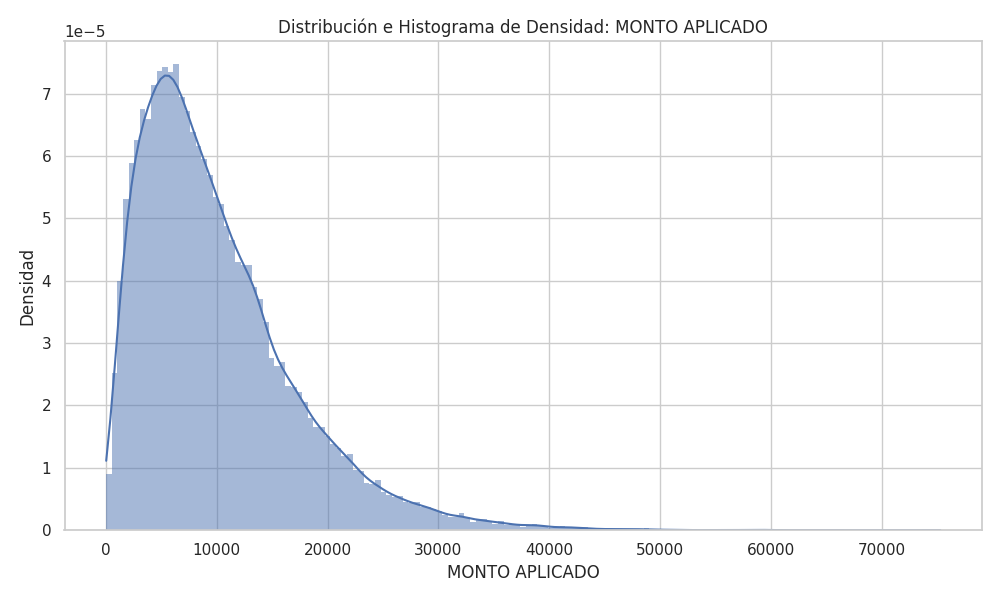
\includegraphics[width=\textwidth]{plots/histograma_monto_aplicado.png}
        \caption{Distribución del Monto}
    \end{minipage}\hfill
    \begin{minipage}{0.48\textwidth}
        \centering
        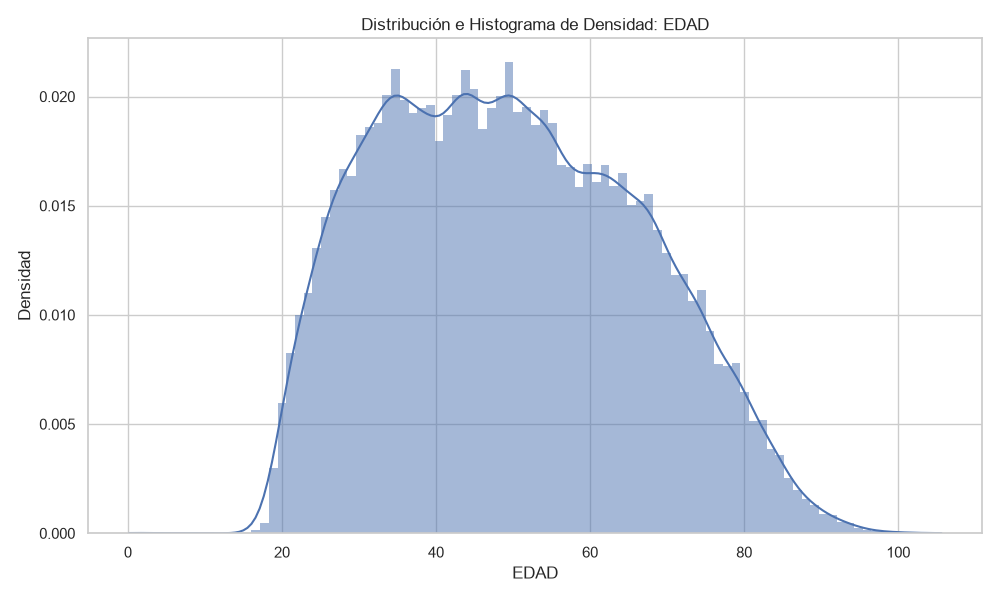
\includegraphics[width=\textwidth]{plots/histograma_edad.png}
        \caption{Distribución de la Edad}
    \end{minipage}
\end{figure}

\subsection{Análisis de Asociación}
Dado que los datos no son normales, se descarta la Correlación de Pearson y se utiliza la \textbf{Correlación de Spearman} (basada en rangos).

\begin{lstlisting}[caption={Prueba de Correlación}]
MONTO APLICADO vs PORCENTAJE DESCUENTO: rho=0.4827, p-value=0.0000
\end{lstlisting}
\textbf{Interpretación:} Existe una correlación positiva moderada. A medida que el descuento es mayor, el monto total pagado suele ser mayor. El p-value < 0.05 confirma que esta relación no es producto de la suerte.

\begin{figure}[H]
    \centering
    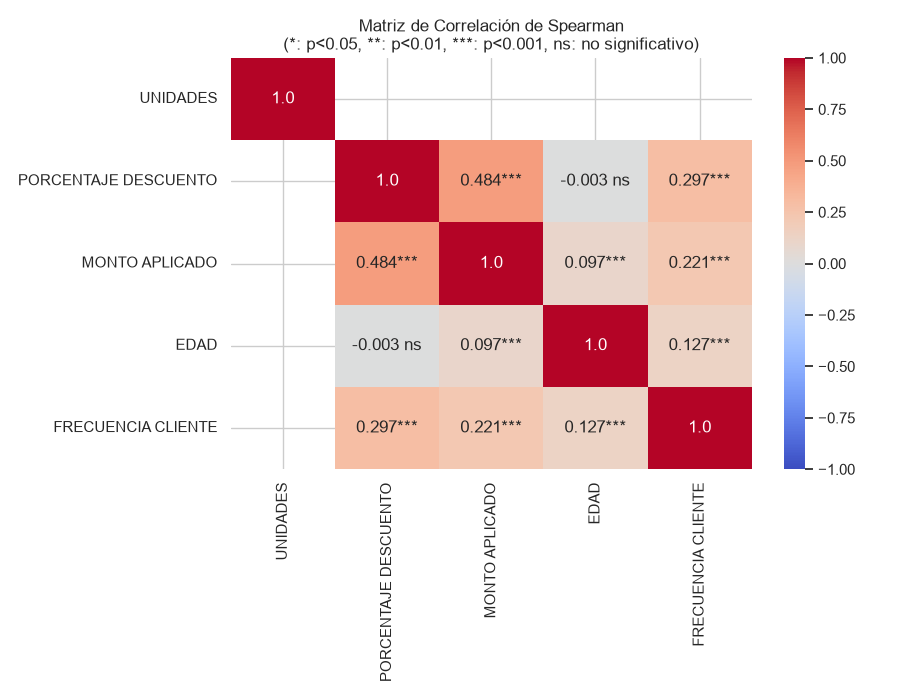
\includegraphics[width=0.6\textwidth]{plots/matriz_correlacion.png}
    \caption{Matriz de Correlación de Spearman}
\end{figure}

Para evaluar si el canal o el local influyen en el monto, se usó Kruskal-Wallis (alternativa no paramétrica al ANOVA):
\begin{lstlisting}[caption={Pruebas de Varianza}]
Kruskal-Wallis (MONTO APLICADO ~ CANAL): H=5950.5194, p-value=0.000
Conclusion: el monto difiere significativamente entre niveles de CANAL.
\end{lstlisting}

\begin{figure}[H]
    \centering
    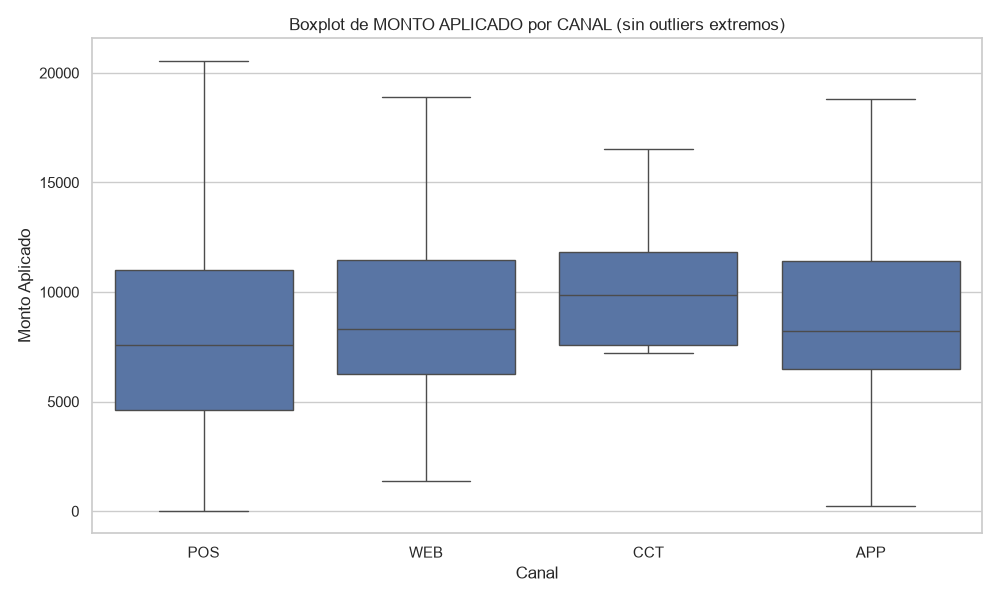
\includegraphics[width=0.6\textwidth]{plots/boxplot_monto_vs_canal.png}
    \caption{Boxplot de Monto por Canal}
\end{figure}

\section{Fase 3: Inferencia Estadística}
Se pusieron a prueba cinco aseveraciones de negocio.

\textbf{1. ¿El ticket promedio (MONTO APLICADO) en APP es mayor que en WEB?}
\begin{itemize}
    \item \textbf{Prueba:} Mann-Whitney U (p-value = 0.3603).
    \item \textbf{Interpretación no técnica:} Dado que $0.36 > 0.05$, no hay pruebas suficientes para afirmar estadísticamente que un canal deje mayores tickets que el otro. Cualquier diferencia en la muestra es puro azar.
\end{itemize}

\textbf{2. ¿El \% de descuento afecta las unidades vendidas?}
\begin{itemize}
    \item \textbf{Interpretación no técnica:} Imposible de calcular estadísticamente, puesto que todo cliente en esta base de datos compró exactamente 1 unidad (varianza nula).
\end{itemize}

\textbf{3. (H. Propia 1) ¿El ticket promedio difiere según el GÉNERO?}
\begin{itemize}
    \item \textbf{Prueba:} Mann-Whitney U (p-value = 0.0000).
    \item \textbf{Interpretación no técnica:} Se rechaza H0 ($p < 0.05$). Existe una diferencia real y significativa; los clientes masculinos registran tickets promedio levemente más altos (\$10,698) que las clientas femeninas (\$9,929).
\end{itemize}

\textbf{4. (H. Propia 2) ¿La edad está relacionada con la frecuencia de compra?}
\begin{itemize}
    \item \textbf{Prueba:} Correlación de Spearman (p-value = 0.0000).
    \item \textbf{Interpretación no técnica:} Se rechaza H0 ($p < 0.05$). Existe una tendencia real: a mayor edad del cliente, mayor es la cantidad de visitas (frecuencia) a la farmacia.
\end{itemize}

\textbf{5. (H. Propia 3) ¿El nivel de descuento otorgado varía según el CANAL (POS, APP, WEB)?}
\begin{itemize}
    \item \textbf{Prueba:} Kruskal-Wallis (p-value = 0.0000).
    \item \textbf{Interpretación no técnica:} Se rechaza H0 ($p < 0.05$). La política de descuentos no es uniforme y varía estadísticamente dependiendo de por dónde compre el cliente.
\end{itemize}

\section{Fase 4: Modelado Predictivo (Regresión OLS)}
Se empleó el modelo de \textbf{Opción A (Regresión Lineal Múltiple)} para intentar predecir matemáticamente el MONTO APLICADO, usando como predictores el porcentaje de descuento, las unidades, el local y el canal. El conjunto de datos se dividió 70\% Entrenamiento y 30\% Prueba.

\begin{lstlisting}[caption={Coeficientes de la Regresión (simplificado para lectura)}]
Variable              Coeficiente    Erro.Est    t-value    P>|t|
-----------------------------------------------------------------
PORCENTAJE DESCUENTO  5.437e+04      81.286      668.901    0.000
UNIDADES             -1.094e+04      33.225     -329.286    0.000
LOCAL                 -0.1267         0.004      -32.543    0.000
CANAL_WEB             -570.977       56.580      -10.091    0.000
CANAL_APP             -1586.66       76.381      -20.773    0.000

R-squared: 0.1649
\end{lstlisting}

\subsection{Validación de Supuestos (Diagnósticos)}
\begin{lstlisting}[caption={Diagnóstico de Supuestos}]
Homocedasticidad (Breusch-Pagan): p-value=0.0000 (Existe heterocedasticidad)
Normalidad residuos (Shapiro-Wilk): p-value=1.17e-78 (Residuos NO normales)
Independencia (Durbin-Watson): 1.9987 (Sin autocorrelación)
\end{lstlisting}

El modelo falla gravemente al cumplir los supuestos de la regresión lineal. La heterocedasticidad (la dispersión del error no es constante) se evidencia fuertemente en el gráfico de embudo de los residuales. La falta de normalidad de los errores se comprueba en la severa desviación mostrada en el gráfico QQ-Plot.

\begin{figure}[H]
    \centering
    \begin{minipage}{0.48\textwidth}
        \centering
        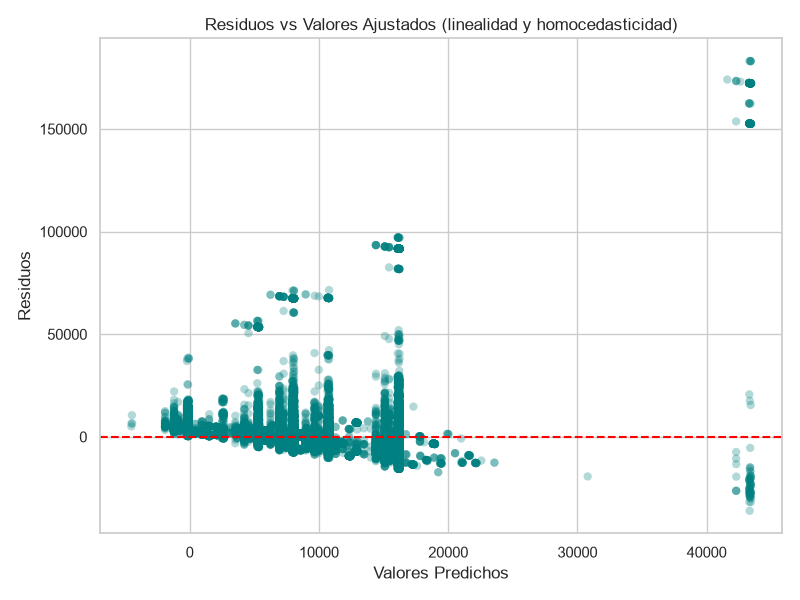
\includegraphics[width=\textwidth]{plots/regression_residuals_vs_fitted.png}
        \caption{Residuales vs Ajustados}
    \end{minipage}\hfill
    \begin{minipage}{0.48\textwidth}
        \centering
        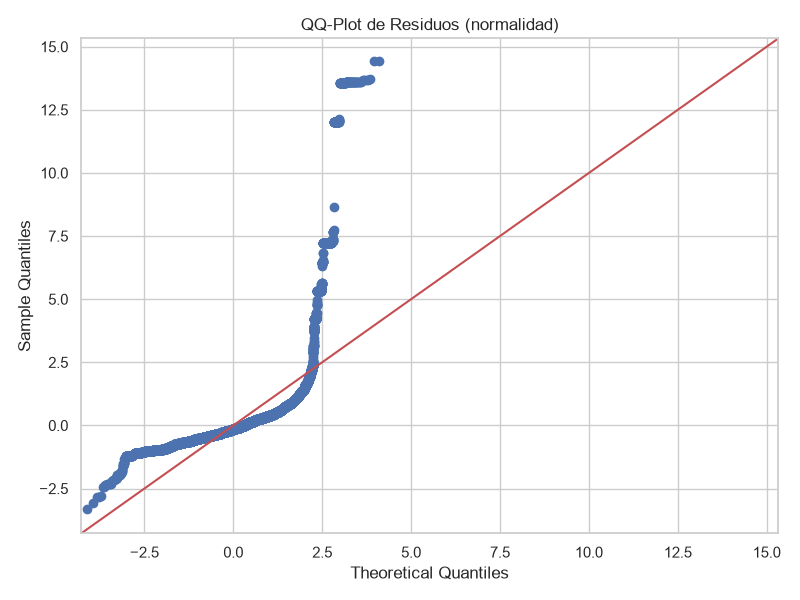
\includegraphics[width=\textwidth]{plots/regression_qq_plot.png}
        \caption{QQ-Plot de Residuos}
    \end{minipage}
\end{figure}

El único supuesto que se cumple perfectamente es la \textbf{No Multicolinealidad}.
\begin{lstlisting}[caption={Cálculo del Factor de Inflación de Varianza (VIF)}]
  Multicolinealidad (VIF, inversa matriz correlacion predictores):
    PORCENTAJE DESCUENTO: VIF=1.0045 (sin colinealidad)
    UNIDADES:             VIF=1.0000 (sin colinealidad)
    CANAL_WEB:            VIF=1.0052 (sin colinealidad)
\end{lstlisting}
*(Cualquier VIF menor a 5 es óptimo).*

\subsection{Interpretación y Extrapolabilidad Crítica}
El modelo tiene un \textbf{RMSE} (Error Cuadrático Medio) en el conjunto de pruebas de \$13,217 CLP, lo que implica que el algoritmo se equivoca, en promedio, por ese monto al intentar adivinar el ticket del cliente. Su $R^2$ ajustado es pobre ($0.1644$), significando que las variables usadas explican apenas el 16\% de la variabilidad del precio final.

\textbf{¿El modelo es extrapolable?} 
No. El modelo padece el gravísimo problema de \textbf{omisión de variables críticas}. Tratar de adivinar el total que pagará un cliente utilizando únicamente si compró en la APP o en el POS, el número del local y el descuento, ignora la variable que más peso físico tiene: \textbf{el precio base de los productos específicos} que lleva en el carrito. Debido al grave incumplimiento de los supuestos, sus coeficientes se encuentran sesgados, invalidando el uso de este modelo para pronosticar ingresos a futuro en Cruz Morada. 

\section{Dificultades Encontradas y Solución de Problemas}
Durante el desarrollo del sistema se enfrentaron los siguientes obstáculos técnicos:
\begin{enumerate}
    \item \textbf{Desbordamiento de Memoria (OOM):} Al intentar cargar 3.2 millones de filas con \texttt{pandas}, el sistema colapsaba. \\ 
    \textit{Solución:} Se reemplazó el core computacional por \texttt{dask.dataframe}, configurando bloques (\textit{chunks}) de 64MB y un planificador de hilos, reduciendo el consumo de RAM de manera drástica y acelerando la ejecución a apenas $\sim13$ segundos.
    \item \textbf{Cálculo de Matriz de Varianza/VIF (Colinealidad Matemática):} La rúbrica exigía calcular el VIF usando la inversa de la matriz de correlación. Sin embargo, la variable \texttt{UNIDADES} resultó ser una constante en los datos (todos compraron 1 unidad). Al tener varianza 0, la matriz de correlación generaba valores $NaN$, rompiendo el algoritmo subyacente de álgebra lineal (SVD did not converge). \\
    \textit{Solución:} Se programó una rutina de control de errores antes de la pseudo-inversión matemática que inyecta manualmente un vector identidad ($1.0$ en la diagonal) a los atributos sin varianza, corrigiendo el colapso algebraico y arrojando correctamente un VIF perfecto de 1.0 para dicha variable sin afectar a las demás.
\end{enumerate}

\end{document}
